\chapter{Radicals, Carbenes and Rearrangements}\label{ch:b3:radicals-carbenes}

The pyrethrum daisy defends itself with esters of chrysanthemic acid, molecules
built around a three-membered carbon ring; their synthetic relatives are among
the most used household insecticides. Chemists close such rings in one step by
adding a \omterm{def:b3:organometallic-bonding:carbene}{carbene} to a double bond: a carbon atom with only six electrons
around it, two of them unshared. This chapter deals with reactive intermediates
that the Year 1 and Year 2 volumes met only in passing (radicals used in
synthesis, \omterm{def:b3:organometallic-bonding:carbene}{carbenes} and \omterm{def:b3:radicals-carbenes:nitrene}{nitrenes}) and with the rearrangements in which a group
moves to an electron-deficient carbon, nitrogen or oxygen atom, among them two
that make the monomers of nylon-6 and of a biodegradable polyester from the
same ketone.

\begin{recall}
The Year 1 volume introduced radicals, homolysis and half-headed arrows,
carbocations and their rearrangements, nucleophiles and leaving groups; the
Year 2 volume radical chains (initiation, propagation, termination, radical
initiators), peroxy acids, lactones, lactams and imines.
\Cref{ch:b3:complex-kinetics} treated chain kinetics,
\cref{ch:b3:organometallic-bonding} \omterm{def:b3:organometallic-bonding:carbene}{carbenes} as ligands,
\cref{ch:b3:many-electron-atoms} singlet and \omterm{def:b3:many-electron-atoms:singlet-triplet}{triplet states}, and
\cref{ch:b3:rate-theories} the Hammond postulate.
\end{recall}

\begin{omfigure}
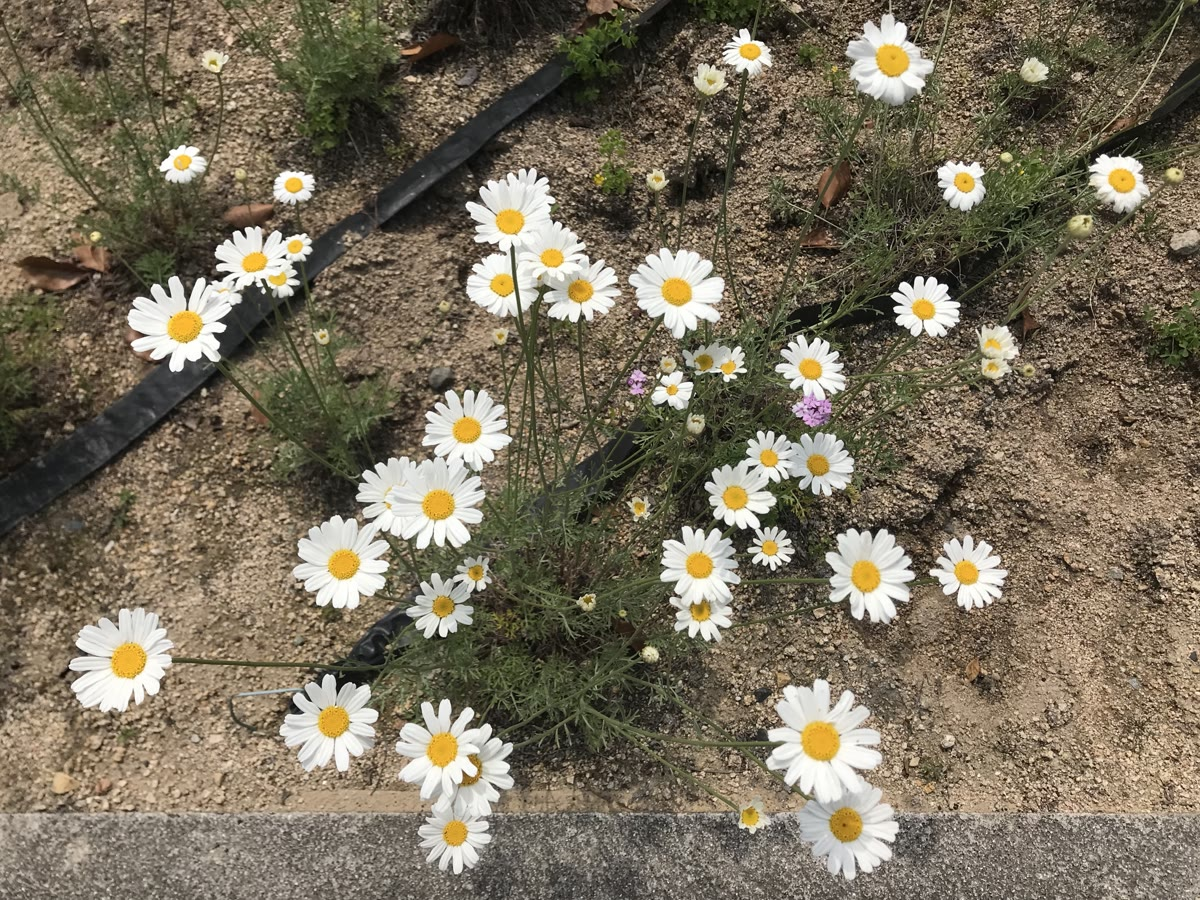
\includegraphics[width=0.48\linewidth]{images/book4/pyrethrum.jpg}

{\small Pyrethrum daisies. Their flowers contain the pyrethrins, insecticidal
esters of a cyclopropanecarboxylic acid. Photograph: Soramimi, CC BY-SA 4.0.}
\end{omfigure}

\section{Radical chain reactions in synthesis}

The stability of a carbon radical is measured by the bond dissociation
enthalpy of the C--H bond that would form it: the weaker the bond, the more
stable the radical.

\begin{proposition}[Bond dissociation enthalpies]\label{prop:b3:radicals-carbenes:bde}
The bond dissociation enthalpy of R--H at \qty{298}{K} follows from gas-phase enthalpies
of formation: $\mathrm{BDE(R{-}H)} = \Delta_fH^\circ(\mathrm R^\bullet) + \Delta_fH^\circ(\mathrm H^\bullet) - \Delta_fH^\circ(\mathrm{RH})$.
\end{proposition}

\begin{proof}
The homolysis $\mathrm{RH \to R^\bullet + H^\bullet}$ has, by Hess's law, the reaction enthalpy of the products'
formation minus that of the reactant; that reaction enthalpy is the bond
dissociation enthalpy by definition.
\end{proof}

\begin{omfigure}
% ledger: dfh4:CH3r, dfh4:C2H5r, dfh4:iC3H7r, dfh4:tC4H9r, dfh4:PhCH2r, dfh4:H, dfh:CH4_g, dfh:C2H6_g, dfh:C3H8_g, dfh4:iC4H10, dfh4:toluene_g
\begin{tikzpicture}
\begin{axis}[width=0.72\linewidth, height=5.2cm, ybar, bar width=16pt, ymin=350, ymax=450,
  xtick={1,2,3,4,5}, xticklabels={{$\ce{CH3-H}$}, {$\ce{C2H5-H}$}, {$\mathrm{(CH_3)_2CH{-}H}$}, {$\mathrm{(CH_3)_3C{-}H}$}, {$\ce{C6H5CH2-H}$}},
  x tick label style={font=\scriptsize}, ylabel={BDE / \unit{kJ.mol^{-1}}},
  axis lines=left, tick label style={font=\scriptsize}, label style={font=\small},
  nodes near coords, nodes near coords style={font=\scriptsize, /pgf/number format/fixed, /pgf/number format/precision=0},
  enlarge x limits=0.15]
\addplot[fill=omDef!55, draw=omDef] table[x=i, y=bde] {figdata/out/bachelor-3-bde.dat};
\end{axis}
\end{tikzpicture}

{\small C--H bond dissociation enthalpies at \qty{298}{K}, computed from gas-phase
enthalpies of formation of the molecules and radicals: methyl, primary,
secondary, tertiary and benzylic. The bond weakens as the radical formed is
more substituted or conjugated.}
\end{omfigure}

\begin{proposition}[Selectivity of halogenation]\label{prop:b3:radicals-carbenes:halogenation-selectivity}
Hydrogen abstraction by a bromine atom is far more selective between primary,
secondary and tertiary C--H bonds than abstraction by a chlorine atom.
\end{proposition}

\begin{proof}[Argued]
With $\mathrm{BDE(H{-}Cl)}$ larger than all the C--H values of the figure and $\mathrm{BDE(H{-}Br)}$ smaller,
abstraction by chlorine is exothermic, by bromine endothermic. By the Hammond
postulate (\cref{ch:b3:rate-theories}) the chlorine transition state is early,
reactant-like, and feels little of the difference between the radicals formed;
the bromine one is late, product-like, and its activation energy follows most of
the difference in BDE, which the Boltzmann factor turns into large rate ratios.
\end{proof}

Tributyltin hydride reduces alkyl halides by a chain: a tin radical takes the
halogen, the alkyl radical takes a hydrogen atom from the next molecule of
hydride, and a new tin radical is made. The same chain removes a hydroxy group
once it is turned into a thiocarbonyl ester (the Barton--McCombie
deoxygenation), and closes rings. Organotin residues are toxic and hard to
remove; tris(trimethylsilyl)silane and other silanes now often replace the tin
hydride.

\begin{omfigure}
\begin{tikzpicture}[font=\small, >=Stealth]
  \node (a) at (-2.0,0) {$\mathrm{Bu_3Sn^\bullet}$};
  \node (b) at (2.0,0) {$\mathrm{R^\bullet}$};
  \draw[->, thick] (a) to[bend left=35] node[midway, above, font=\scriptsize] {$+\,$R--Br, $\ -\,\mathrm{Bu_3SnBr}$} (b);
  \draw[->, thick] (b) to[bend left=35] node[midway, below, font=\scriptsize] {$+\,\mathrm{Bu_3SnH}$, $\ -\,$R--H} (a);
  \node[font=\scriptsize, align=center, anchor=north] at (0,-1.5) {initiation: AIBN $\xrightarrow{\Delta}$ 2 R$'^\bullet$ $+$ $\ce{N2}$; \ R$'^\bullet$ $+$ $\mathrm{Bu_3SnH}$ $\to$ R$'$H $+$ $\mathrm{Bu_3Sn^\bullet}$};
\end{tikzpicture}

{\small The propagation steps of a tin hydride reduction of an alkyl bromide.
Each R--Br reduced uses one $\mathrm{Bu_3SnH}$ and gives one $\mathrm{Bu_3SnBr}$; the \omterm{def:b3:complex-kinetics:chain}{chain carriers}
are the tin radical and the alkyl radical.}
\end{omfigure}

Hydrogen bromide adds to alkenes by the same kind of chain when peroxides are
present: a bromine atom adds to the less substituted end, giving the more
stable radical, which then takes a hydrogen atom from HBr: anti-Markovnikov
addition.

\section{Radical cyclisations}

\begin{definition}[Exo and endo cyclisations]\label{def:b3:radicals-carbenes:cyclisation}
In an \emph{exo cyclisation}\index{exo cyclisation} the bond that is broken (or
the $\pi$ bond attacked) ends up outside the new ring; in an \emph{endo
cyclisation}\index{endo cyclisation}, inside it.
\end{definition}

\begin{omfigure}
\begin{tikzpicture}[font=\scriptsize, >=Stealth]
  % hex-5-enyl radical: C1 radical, C5=C6
  \foreach \i/\a in {1/162, 2/234, 3/306, 4/18} { \coordinate (p\i) at (\a:0.9); }
  \coordinate (p5) at (90:0.95); \coordinate (p6) at (90:1.9);
  \draw[thick] (p1) -- (p2) -- (p3) -- (p4) -- (p5);
  \draw[thick, double, double distance=1.5pt] (p5) -- (p6);
  \node[anchor=east] at (p1) {$\bullet$\,1};
  \node[anchor=west] at (p5) {5}; \node[anchor=west] at (p6) {6};
  \draw[->, omMeth, thick] ($(p1)+(0.1,0.15)$) to[bend left=25] node[pos=0.45, below right, inner sep=1pt] {5-exo} ($(p5)+(-0.15,-0.05)$);
  \draw[->, omThm, thick, densely dashed] ($(p1)+(0,0.25)$) to[bend left=50] node[midway, left] {6-endo} ($(p6)+(-0.2,0)$);
  \node[font=\small, align=center] at (0,-1.6) {hex-5-enyl radical};
  \draw[->, thick] (1.6,0.3) -- (2.7,0.3) node[midway, above] {fast};
  \begin{scope}[xshift=4.0cm]
    \foreach \i/\a in {1/162, 2/234, 3/306, 4/18, 5/90} { \coordinate (q\i) at (\a:0.75); }
    \draw[thick] (q1) -- (q2) -- (q3) -- (q4) -- (q5) -- (q1);
    \draw[thick] (q5) -- ++(90:0.6) coordinate (q6);
    \node[anchor=south, inner sep=1pt] at (q6) {$\mathrm{{}^\bullet CH_2}$};
    \node[font=\small, align=center] at (0,-1.6) {cyclopentylmethyl radical};
  \end{scope}
\end{tikzpicture}

{\small The 5-hexenyl radical closes by attack of C1 on C5 (5-exo, green): the
new ring has five members and the radical ends outside it, on C6. Attack on C6
(6-endo, red dashed) would give the more stable secondary cyclohexyl radical
but is much slower: the chain cannot place C1 on the line of approach to C6 that
the $\pi^*$ orbital requires.}
\end{omfigure}

\begin{proposition}[Baldwin's rules]\label{prop:b3:radicals-carbenes:baldwin}
For ring closures (established experimentally, with a stereoelectronic
rationale): at a tetrahedral carbon (tet), 3- to 7-exo are favoured, 5- and
6-endo disfavoured; at a trigonal carbon (trig), 3- to 7-exo are favoured, 3- to 5-endo
disfavoured, 6- and 7-endo favoured; at a digonal carbon (dig), 3- and 4-exo are
disfavoured, 5- to 7-exo favoured, 3- to 7-endo favoured.
\end{proposition}

The rationale is the angle of attack each kind of bond needs: from the back of
the bond at a tet carbon, at about 107° to a trigonal $\pi$ system, at a narrower
angle to a triple bond; a short chain cannot reach those positions for the
disfavoured cases.

\begin{definition}[Radical clock]\label{def:b3:radicals-carbenes:radical-clock}
A \emph{radical clock}\index{radical clock} is a radical that rearranges
unimolecularly with a known rate constant, such as the 5-hexenyl radical
cyclising; its competition with a bimolecular trap measures the rate constant
of the trap, or the reverse.
\end{definition}

\begin{proposition}[Competition kinetics]\label{prop:b3:radicals-carbenes:clock}
If a radical either cyclises ($k_c$) or is trapped by a hydride kept in excess at
concentration $[\mathrm{R_3SnH}]$ ($k_H$), the product ratio is
$[\text{cyclised}]/[\text{direct}] = k_c/(k_H[\mathrm{R_3SnH}])$.
\end{proposition}

\begin{proof}
At every moment the two products form at rates $k_c[\mathrm R^\bullet]$ and $k_H[\mathrm{R_3SnH}][\mathrm R^\bullet]$. Their ratio
does not depend on the radical concentration, which varies; with the hydride
concentration constant, integration over time multiplies both by the same
$\int[\mathrm R^\bullet]\,\dd t$, and the ratio of the products is the ratio of the rate constants
times $1/[\mathrm{R_3SnH}]$.
\end{proof}

\begin{omfigure}
\begin{tikzpicture}
\begin{axis}[name=a, width=0.47\linewidth, height=5.2cm, xmode=log, xmin=1e-3, xmax=1, ymin=0, ymax=1,
  axis lines=left, xlabel={$[\mathrm{Bu_3SnH}]$ / \unit{mol.L^{-1}}}, ylabel={fraction cyclised},
  tick label style={font=\scriptsize}, label style={font=\small}]
\addplot[omDef, thick] table[x=c, y=fcyc] {figdata/out/bachelor-3-radical-clock.dat};
\end{axis}
\begin{axis}[at={(a.east)}, anchor=west, xshift=1.5cm, width=0.47\linewidth, height=5.2cm,
  xmin=0, xmax=1, ymin=0, ymax=11, axis lines=left,
  xlabel={$[\mathrm{Bu_3SnH}]$ / \unit{mol.L^{-1}}}, ylabel={[direct]/[cyclised]},
  tick label style={font=\scriptsize}, label style={font=\small}]
\addplot[omThm, thick] table[x=c, y=inv] {figdata/out/bachelor-3-radical-clock-b.dat};
\node[font=\scriptsize, anchor=west, omThm] at (axis cs:0.15,7.5) {slope $k_H/k_c$};
\end{axis}
\end{tikzpicture}

{\small The 5-hexenyl clock with model rate constants $k_c = \qty{2.3e5}{s^{-1}}$ and
$k_H = \qty{2.4e6}{L.mol^{-1}.s^{-1}}$. Left: fraction of methylcyclopentane among the products against the
hydride concentration: half at $k_c/k_H \approx \qty{0.1}{mol/L}$. Right: the inverse ratio is a straight
line through the origin, of slope $k_H/k_c$.}
\end{omfigure}

\begin{method}[Designing a radical reduction or cyclisation]\label{met:b3:radicals-carbenes:radical-chain}
\begin{enumerate}
  \item For a simple reduction, keep the hydrogen donor concentrated (about
        \qty{0.1}{mol/L} or more) so that the radical is trapped before it rearranges.
  \item For a cyclisation, keep the donor dilute, or add it slowly, so that the
        radical cyclises first: choose $[\text{donor}] \ll k_c/k_H$.
  \item Choose an initiator whose half-life at the reaction temperature is of the
        order of the reaction time (AIBN near \qty{80}{\celsius}), and add it in portions if
        needed.
  \item Prefer a silane or another tin-free donor, and remove oxygen, which traps
        carbon radicals.
\end{enumerate}
\end{method}

\begin{inthelab}[Slow addition with a syringe pump]
To keep a reagent dilute throughout a reaction, its solution is loaded into a
gas-tight syringe and added through a septum by a syringe pump over several
hours, into the refluxing solution of the substrate under nitrogen. The
concentration of the reagent then stays near its low steady-state value, set by
the rate of addition and the rate at which it is consumed.
\end{inthelab}

\section{Carbenes}

\begin{definition}[Singlet and triplet carbenes]\label{def:b3:radicals-carbenes:carbene-states}
A \emph{singlet carbene}\index{singlet carbene} has its two non-bonding
electrons paired in one orbital, an $sp^2$ hybrid, its p orbital empty; a
\emph{triplet carbene}\index{triplet carbene} has them unpaired, one in each
orbital, with parallel spins.
\end{definition}

\begin{omfigure}
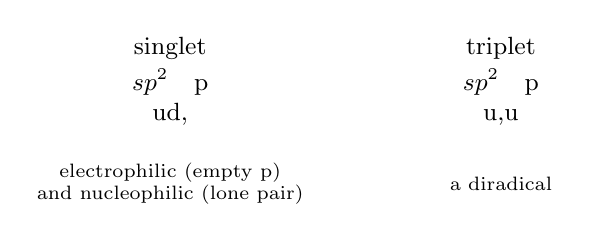
\begin{tikzpicture}[font=\small]
  \node[align=center] at (0,0) {singlet\\[2pt] $sp^2$ \ \ p\\ \omorbs{ud,}};
  \node[align=center] at (4.2,0) {triplet\\[2pt] $sp^2$ \ \ p\\ \omorbs{u,u}};
  \node[font=\scriptsize, align=center] at (0,-1.3) {electrophilic (empty p)\\ and nucleophilic (lone pair)};
  \node[font=\scriptsize, align=center] at (4.2,-1.3) {a diradical};
\end{tikzpicture}

{\small Electron occupations of the two non-bonding orbitals of a \omterm{def:b3:organometallic-bonding:carbene}{carbene}. The
triplet is the ground state of $\ce{CH2}$; $\pi$-donor substituents (Cl, OR, $\mathrm{NR_2}$) raise the
p orbital and make the singlet the ground state, as in dichlorocarbene.}
\end{omfigure}

\omterm{def:b3:organometallic-bonding:carbene}{Carbenes} are made by losing dinitrogen from a diazo compound (by heat, light
or a metal catalyst), by $\alpha$-elimination (chloroform and a strong base give
$\ce{CCl3-}$, which loses chloride to $\ce{CCl2}$), or are avoided altogether by a
\omterm{def:b3:radicals-carbenes:carbenoid}{carbenoid}.

\begin{definition}[Carbenoids]\label{def:b3:radicals-carbenes:carbenoid}
A \emph{carbenoid}\index{carbenoid} is a metal-bound species that transfers a
\omterm{def:b3:organometallic-bonding:carbene}{carbene} group as a free \omterm{def:b3:organometallic-bonding:carbene}{carbene} would, without the free \omterm{def:b3:organometallic-bonding:carbene}{carbene} being formed,
such as the iodomethylzinc iodide $\ce{ICH2ZnI}$ of the Simmons--Smith reaction.
\end{definition}

\begin{definition}[Cyclopropanation]\label{def:b3:radicals-carbenes:cyclopropanation}
\emph{Cyclopropanation}\index{cyclopropanation} is the formation of a
cyclopropane by addition of a \omterm{def:b3:organometallic-bonding:carbene}{carbene} or \omterm{def:b3:radicals-carbenes:carbenoid}{carbenoid} to a C=C double bond.
\end{definition}

\begin{proposition}[The Skell test]\label{prop:b3:radicals-carbenes:skell}
A \omterm{def:b3:radicals-carbenes:carbene-states}{singlet carbene} adds to a \textit{cis} or \textit{trans} alkene stereospecifically, keeping the
relative configuration; a \omterm{def:b3:radicals-carbenes:carbene-states}{triplet carbene} gives both cyclopropane
stereoisomers.
\end{proposition}

\begin{proof}[Argued]
The singlet makes both new bonds in one concerted step, with no time for
rotation. The triplet makes one bond first, giving a triplet 1,3-diradical; its
two unpaired electrons cannot form the second bond until a spin flips, which is
slow compared with rotation about the remaining C--C single bond: the
configuration is scrambled.
\end{proof}

\begin{omfigure}
\setchemfig{atom sep=1.8em}
\schemestart
\chemfig{H_3C-[:30]=[:0]-[:-30]CH_3}
\arrow{->[singlet $\ce{CH2}$]}[,1.6]
\chemfig{(<[:210]H_3C)-[:0](<[:330]CH_3)-[:120]-[:240]}
\schemestop
\par\medskip

{\small Skell's test: \textit{cis}-but-2-ene, both methyl groups on the same side, gives with
a \omterm{def:b3:radicals-carbenes:carbene-states}{singlet carbene} only \textit{cis}-1,2-dimethylcyclopropane (both methyl groups on wedges,
on the same face of the ring); with a \omterm{def:b3:radicals-carbenes:carbene-states}{triplet
carbene} the \textit{trans} isomer appears too.}
\end{omfigure}

\omterm{def:b3:radicals-carbenes:carbene-states}{Singlet carbenes} also insert into C--H bonds. Rhodium(II) carboxylates
decompose diazo esters into rhodium \omterm{def:b3:radicals-carbenes:carbenoid}{carbenoids} that cyclopropanate alkenes and
insert into C--H bonds selectively, and, with chiral ligands, enantioselectively.

\begin{definition}[Nitrenes]\label{def:b3:radicals-carbenes:nitrene}
A \emph{nitrene}\index{nitrene} $\mathrm{R{-}\ddot N}$ is the nitrogen analogue of a \omterm{def:b3:organometallic-bonding:carbene}{carbene}, a neutral
nitrogen atom with only six electrons, formed for example by loss of
dinitrogen from an azide.
\end{definition}

\section{Rearrangements to electron-deficient carbon}

\begin{definition}[1,2-Shift]\label{def:b3:radicals-carbenes:shift}
A \emph{1,2-shift}\index{1,2-shift} is the migration of a group, with its bonding
pair, from one atom to the neighbouring electron-deficient atom.
\end{definition}

In a Wagner--Meerwein shift an alkyl group or a hydride moves to a neighbouring
carbocation, giving a more stable one: the carbocation rearrangements of the
Year 1 volume, now with their mechanism named. Terpene skeletons are reshaped
in nature by cascades of such shifts.

\begin{definition}[Pinacol rearrangement]\label{def:b3:radicals-carbenes:pinacol}
The \emph{pinacol rearrangement}\index{pinacol rearrangement} turns a 1,2-diol,
in acid, into a ketone or an aldehyde: one hydroxy group leaves as water, a
group on the neighbouring carbon shifts to the cation, and the cation formed,
stabilised by the remaining oxygen, loses a proton.
\end{definition}

\begin{definition}[Migratory aptitude]\label{def:b3:radicals-carbenes:migratory}
The \emph{migratory aptitude}\index{migratory aptitude} of a group is its
relative tendency to move in a \omterm{def:b3:radicals-carbenes:shift}{1,2-shift} to an electron-deficient centre.
\end{definition}

Groups that carry positive charge well during the shift migrate best: hydride,
aryl and tertiary alkyl before secondary, primary and methyl. Pinacol,
$\mathrm{(CH_3)_2C(OH){-}C(OH)(CH_3)_2}$, gives pinacolone, 3,3-dimethylbutan-2-one.

\begin{method}[Predicting the product of a rearrangement]\label{met:b3:radicals-carbenes:rearrangement}
\begin{enumerate}
  \item Find the electron-deficient atom formed (cation, nitrenium, oxygen of an
        activated peroxide, \omterm{def:b3:organometallic-bonding:carbene}{carbene} or \omterm{def:b3:radicals-carbenes:nitrene}{nitrene}) and the leaving group that makes
        it.
  \item List the groups on the neighbouring atom that could move; when the
        geometry is fixed (oximes), only the group anti to the leaving group can.
  \item Otherwise choose by \omterm{def:b3:radicals-carbenes:migratory}{migratory aptitude}, or by which group forms the more
        stable cation where it leaves.
  \item Move the group with retention of its configuration, then complete the
        mechanism (loss of a proton, addition of water).
\end{enumerate}
\end{method}

\section{Rearrangements to electron-deficient nitrogen and oxygen}

\begin{definition}[Beckmann rearrangement]\label{def:b3:radicals-carbenes:beckmann}
The \emph{Beckmann rearrangement}\index{Beckmann rearrangement} turns an oxime,
in strong acid, into an amide: the hydroxy group, activated as a leaving group,
departs while the group anti to it migrates from carbon to nitrogen; water adds
to the nitrilium ion formed, and tautomerisation gives the amide.
\end{definition}

\begin{proposition}[Anti migration]\label{prop:b3:radicals-carbenes:beckmann-anti}
In the \omterm{def:b3:radicals-carbenes:beckmann}{Beckmann rearrangement} the group that migrates is the one anti to the
leaving group on nitrogen.
\end{proposition}

\begin{proof}[Argued]
The migrating bond pair attacks nitrogen from the back of the N--O bond, as in an
$\mathrm S_\mathrm N2$ displacement; only the group anti to the oxygen has its bond aligned with
the N--O $\sigma^*$ orbital. The step is concerted with the departure of the leaving group,
so no free nitrenium ion forms that could choose otherwise.
\end{proof}

\begin{omfigure}
\setchemfig{atom sep=1.9em}
\schemestart
\chemfig{*6(-----(=N-[:30]OH)-)}
\arrow{->[$\ce{H2SO4}$ (oleum)][Beckmann]}[,1.8]
\chemfig{*7(---N(-[:-90]H)-(=O)---)}
\schemestop
\par\medskip
\schemestart
\chemfig{*6(-----(=O)-)}
\arrow{->[peroxy acid][Baeyer--Villiger]}[,1.8]
\chemfig{*7(-----O-(=O)-)}
\schemestop

{\small Two ring expansions of cyclohexanone. Top: its oxime rearranges in
oleum to caprolactam (azepan-2-one), the monomer of nylon-6, nitrogen entering
the ring. Bottom: a peroxy acid inserts an oxygen atom next to the carbonyl
group, giving $\varepsilon$-caprolactone (oxepan-2-one).}
\end{omfigure}

\begin{definition}[Baeyer--Villiger oxidation]\label{def:b3:radicals-carbenes:baeyer}
The \emph{Baeyer--Villiger oxidation}\index{Baeyer--Villiger oxidation} turns a
ketone into an ester, or a cyclic ketone into a lactone, with a peroxy acid: the
peroxy acid adds to the carbonyl group, then a group on the carbonyl carbon
migrates to the nearer peroxide oxygen as a carboxylate leaves.
\end{definition}

\begin{proposition}[Baeyer--Villiger regiochemistry]\label{prop:b3:radicals-carbenes:bv-retention}
In the \omterm{def:b3:radicals-carbenes:baeyer}{Baeyer--Villiger oxidation} the group that migrates keeps its
configuration, and the order of \omterm{def:b3:radicals-carbenes:migratory}{migratory aptitude} is tertiary alkyl >
secondary alkyl $\approx$ aryl > primary alkyl > methyl (established experimentally).
\end{proposition}

\begin{proof}[Argued]
The group moves with its bonding pair across the face of the carbon it leaves
and lands on oxygen from the same side, so its configuration is kept. In the
transition state the migrating group carries partial positive charge, which
alkyl substitution and aryl conjugation stabilise.
\end{proof}

\begin{definition}[Isocyanates, Curtius and Hofmann rearrangements]\label{def:b3:radicals-carbenes:curtius}
An \emph{isocyanate}\index{isocyanate} is a compound $\ce{R-N=C=O}$. In the \emph{Curtius rearrangement}
\index{Curtius rearrangement} an acyl azide loses dinitrogen on
heating while the R group moves from carbon to nitrogen, giving an isocyanate;
in the \emph{Hofmann rearrangement}\index{Hofmann rearrangement} a primary amide
treated with bromine and base gives the same isocyanate through an
N-bromoamide. With water the isocyanate gives the amine $\ce{RNH2}$ and carbon
dioxide; with an alcohol, a carbamate.
\end{definition}

\begin{definition}[Ketenes and the Wolff rearrangement]\label{def:b3:radicals-carbenes:wolff}
A \emph{ketene}\index{ketene} is a compound $\mathrm{R_2C{=}C{=}O}$. In the \emph{Wolff rearrangement}
\index{Wolff rearrangement} an $\alpha$-diazoketone loses dinitrogen
while the group on the carbonyl carbon migrates, giving a ketene, which adds
water, an alcohol or an amine.
\end{definition}

The \omterm{def:b3:radicals-carbenes:wolff}{Wolff rearrangement} is the key step of the Arndt--Eistert homologation,
which lengthens a carboxylic acid by one carbon: acid chloride, then
diazoketone, then \omterm{def:b3:radicals-carbenes:wolff}{ketene}, then the homologous acid.

\begin{safety}{\ghs[0.62cm]{GHS06}\ghs[0.62cm]{GHS08}\ghs[0.62cm]{GHS09}}
% ledger: ghs4:Bu3SnH, ghs4:diazomethane, ghs4:AIBN
Tributyltin hydride: toxic if swallowed, harmful on skin, damages organs on
repeated exposure, very toxic to aquatic life; tin residues are collected
separately. Diazomethane is a toxic, carcinogenic and explosive gas; it is
named here for its chemistry only and is replaced in practice by safer reagents
such as trimethylsilyldiazomethane. AIBN is self-reactive on heating.
\end{safety}

\begin{history}[A radical that should not exist, and a nylon]
In 1900 Moses Gomberg, trying to make hexaphenylethane, obtained a yellow
solution that took up oxygen and iodine: the triphenylmethyl radical, the first
persistent carbon radical. Half a century later, the \omterm{def:b3:radicals-carbenes:beckmann}{Beckmann rearrangement} of
cyclohexanone oxime became the industrial route to caprolactam, polymerised by
ring opening into nylon-6, a fibre and engineering plastic made on a very large
scale.
\end{history}

\section{Exercises}

\begin{exercise}[$\star$]\label{exo:b3:radicals-carbenes:1}
At \qty{25}{\celsius} the relative reactivities per hydrogen of primary, secondary and
tertiary C--H bonds are $1 : 3.9 : 5.1$ towards chlorine atoms and $1 : 82 : 1600$ towards
bromine atoms (data of the exercise). Compute the proportions of 1- and 2-halopropane
formed from propane in each case.
\end{exercise}

\begin{exercise}[$\star$]\label{exo:b3:radicals-carbenes:2}
Which is the ground state of $\ce{CH2}$, and of $\ce{CCl2}$? Which adds stereospecifically to
\textit{trans}-but-2-ene, and what does it give?
\end{exercise}

\begin{exercise}[$\star$]\label{exo:b3:radicals-carbenes:3}
Give the product of the Simmons--Smith reaction of (\textit{Z})-hex-3-ene.
\end{exercise}

\begin{exercise}[$\star$]\label{exo:b3:radicals-carbenes:4}
Give the products of the \omterm{def:b3:radicals-carbenes:baeyer}{Baeyer--Villiger oxidation} of cyclohexanone and of
acetophenone.
\end{exercise}

\begin{exercise}[$\star\star$]\label{exo:b3:radicals-carbenes:5}
With the data of \cref{exo:b3:radicals-carbenes:1}, compute the proportions of
the two monochlorides and of the two monobromides of 2-methylpropane.
\end{exercise}

\begin{exercise}[$\star\star$]\label{exo:b3:radicals-carbenes:6}
A new \omterm{def:b3:radicals-carbenes:radical-clock}{radical clock}, reduced with $\qty{0.020}{mol/L}$ $\mathrm{Bu_3SnH}$, gives three times as much rearranged
as unrearranged product. With $k_H = \qty{2.4e6}{L.mol^{-1}.s^{-1}}$, find its rate constant.
\end{exercise}

\begin{exercise}[$\star\star$]\label{exo:b3:radicals-carbenes:7}
Classify by Baldwin's rules the attack of a hex-5-enyl radical on C5 and on C6,
then say whether each of these closures is favoured: 4-exo-tet, 5-endo-trig,
5-exo-dig, 3-exo-dig, 5-endo-dig.
\end{exercise}

\begin{exercise}[$\star\star$]\label{exo:b3:radicals-carbenes:8}
Give the product of the \omterm{def:b3:radicals-carbenes:pinacol}{pinacol rearrangement} of 2,3-diphenylbutane-2,3-diol,
and explain the choice of the migrating group.
\end{exercise}

\begin{exercise}[$\star\star$]\label{exo:b3:radicals-carbenes:9}
Benzoyl azide is heated in toluene, then water is added; in a second experiment,
ethanol. Give the products.
\end{exercise}

\begin{exercise}[$\star\star\star$]\label{exo:b3:radicals-carbenes:10}
With $\mathrm{BDE(H{-}Cl)} = \qty{432}{kJ/mol}$ and $\mathrm{BDE(H{-}Br)} = \qty{366}{kJ/mol}$ (data of the exercise) and the C--H values of
the chapter's figure, compute $\Delta H$ for abstraction of a primary and of a tertiary
hydrogen by each halogen atom, and use the Hammond postulate to explain the
selectivities of \cref{exo:b3:radicals-carbenes:1}.
\end{exercise}

\begin{exercise}[$\star\star\star$]\label{exo:b3:radicals-carbenes:11}
Give the Beckmann products of the two oximes, \textit{E} and \textit{Z}, of 2-methylcyclohexanone,
and explain why they differ, while the \omterm{def:b3:radicals-carbenes:baeyer}{Baeyer--Villiger oxidation} of the
ketone gives one main lactone.
\end{exercise}

\begin{exercise}[$\star\star\star$]\label{exo:b3:radicals-carbenes:12}
With the model clock of the chapter, compute the fraction cyclised at $[\mathrm{Bu_3SnH}] = 0.010$,
0.10 and \qty{1.0}{mol/L}. What hydride concentration gives 95\,\% of cyclised product, and how
can it be maintained?
\end{exercise}

\section{Problem: Two Rings from Cyclohexanone}

\begin{problem}[{Weekend problem --- two rings from cyclohexanone: the oxime, the
Beckmann rearrangement to caprolactam, the Baeyer--Villiger oxidation to
caprolactone, and the regiochemistry of both with 2-methylcyclohexanone}]
\label{pb:b3:radicals-carbenes:1}
% ledger: aw:C, aw:H, aw:N, aw:O, aw:S
Data of the problem: one tonne of cyclohexanone is converted into its oxime with
98\,\% yield, and the oxime into caprolactam with 98\,\% yield; the rearrangement uses
1.3 mol of sulfuric acid (as oleum) per mole of oxime, neutralised at the end with
ammonia to ammonium sulfate.

\medskip\noindent\textbf{Part I --- The oxime.}
\begin{enumerate}
  \item Write the formation of cyclohexanone oxime from hydroxylamine.
  \item Why is it run near pH 4 to 5?
  \item Does cyclohexanone oxime have \textit{E} and \textit{Z} isomers? Why?
  \item Draw the \textit{E} and \textit{Z} oximes of 2-methylcyclohexanone.
  \item Why do these two oximes interconvert only slowly?
\end{enumerate}

\medskip\noindent\textbf{Part II --- The \omterm{def:b3:radicals-carbenes:beckmann}{Beckmann rearrangement}.}
\begin{enumerate}[resume]
  \item What does the acid do to the oxime?
  \item Which bond migrates, and why does it make the ring larger?
  \item What intermediate does water attack?
  \item Write the overall equation, oxime to caprolactam.
  \item Name and draw the product, and the polymer made from it.
  \item Compute the molar masses of cyclohexanone and caprolactam.
  \item Compute the mass of caprolactam from one tonne of cyclohexanone.
  \item Compute the mass of ammonium sulfate made with it.
\end{enumerate}

\medskip\noindent\textbf{Part III --- The \omterm{def:b3:radicals-carbenes:baeyer}{Baeyer--Villiger oxidation}.}
\begin{enumerate}[resume]
  \item Write the oxidation of cyclohexanone by a peroxy acid $\ce{RCO3H}$.
  \item Give the intermediate formed by addition of the peroxy acid.
  \item Which group migrates, and what is the leaving group?
  \item Name the lactone and the polymer it gives.
  \item Why can hydrogen peroxide with a catalyst replace the peroxy acid in a
        cleaner process?
\end{enumerate}

\medskip\noindent\textbf{Part IV --- 2-Methylcyclohexanone.}
\begin{enumerate}[resume]
  \item Which carbon migrates in its \omterm{def:b3:radicals-carbenes:baeyer}{Baeyer--Villiger oxidation}, and what lactone forms?
  \item Is the configuration of that carbon kept?
  \item Which lactam does the \textit{E} oxime give (OH anti to the methyl-bearing carbon)?
  \item Which lactam does the \textit{Z} oxime give?
  \item What decides the regiochemistry in each reaction?
  \item Why is cyclohexanone itself free of these problems?
  \item State the result: the mass of caprolactam from one tonne of cyclohexanone.
\end{enumerate}
\end{problem}
